\subsection{信号的基本运算}

\subsubsection{四则运算}

\begin{definition}
    信号的\bd{四则运算}是指,对信号进行加、减、乘、除等运算。四则运算后的信号在任意一点的取值定义为
    原信号在同一点处函数值作相同四则运算的结果。
    \begin{align*}
        (f_1 + f_2)(t) & = f_1(t) + f_2(t), \\
        (f_1 - f_2)(t) & = f_1(t) - f_2(t), \\
        (f_1 \cdot f_2)(t) & = f_1(t) \cdot f_2(t), \\
        \left(\frac{f_1}{f_2}\right)(t) & = \frac{f_1(t)}{f_2(t)}.
    \end{align*}
\end{definition}

\begin{note}
    四则运算中的乘法\bd{不能用星号 $*$ 表示},因为 $*$ 表示卷积运算。
\end{note}

\subsubsection{波形变换}

\begin{definition}[时移运算]
    信号的\bd{时移运算}是指,将原信号 $f(t)$ 沿横轴平移 $b$ 个单位,
    得到新信号 $f(t - b)$。其中,实参数 $b$ 决定平移方向和位移量。
    \begin{itemize}
        \item $b > 0$ 时,信号向右平移。
        \item $b < 0$ 时,信号向左平移。
    \end{itemize}
\end{definition}

\begin{note}
    可以按照``左加右减''的口诀来记忆时移运算的方向。设有 $b > 0$,
    则 $f(t + b)$ 表示信号向左平移 $b$ 个单位,
    $f(t - b)$ 表示信号向右平移 $b$ 个单位。
\end{note}

\begin{example}
    假设有原信号 $f(t)$,则其时移信号 $f(t + 8)$ 和 $f(t - 9)$ 如图 \ref{fig:waveform-translation} 所示。
    \begin{figure}[H]
        \centering
        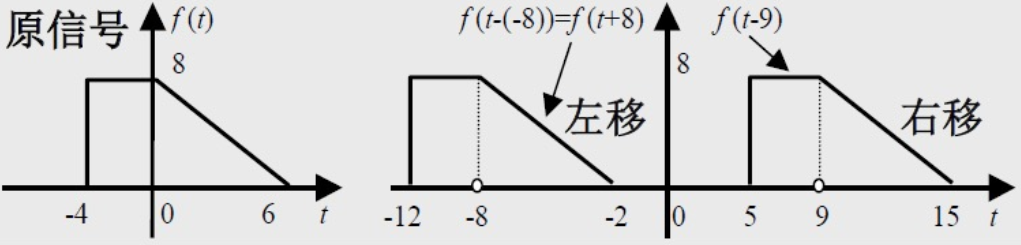
\includegraphics[width=0.5\textwidth]{chap1/img/waveform-translation.png}
        \caption{信号的时移运算}
        \label{fig:waveform-translation}
    \end{figure}
\end{example}

\begin{definition}[反褶运算]
    信号的\bd{反褶运算}是指,将原信号 $f(t)$ 按照纵轴对称翻转过来,
    得到新信号 $f(-t)$。
\end{definition}

\begin{example}
    如图 \ref{fig:waveform-symmetry} 所示,假设有原信号 $f(t)$,
    则其反褶信号为 $f(-t)$。
    \begin{figure}[H]
        \centering
        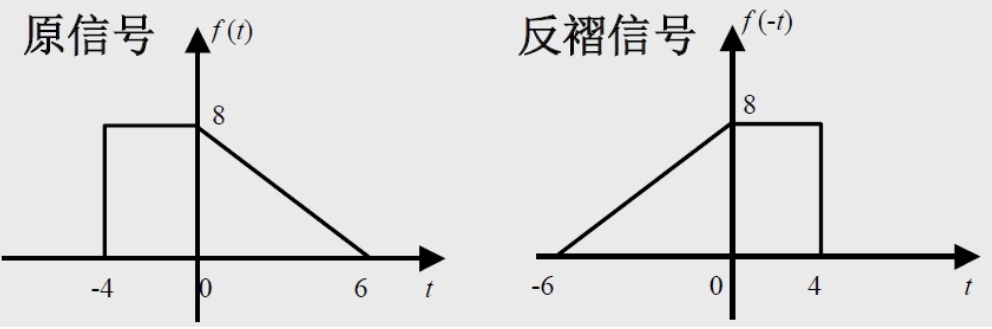
\includegraphics[width=0.5\textwidth]{chap1/img/waveform-symmetry.png}
        \caption{信号的反褶运算}
        \label{fig:waveform-symmetry}
    \end{figure}
\end{example}

\begin{definition}[压扩运算]
    信号的\bd{压扩运算}是指,将原信号 $f(t)$ 沿横轴缩放 $a$ 倍,
    得到新信号 $f(at)$。其中,实参数 $a$ 决定缩放方向和缩放倍数。
    当 $a < 0$ 时,信号需要先进行反褶运算,再进行压扩运算。
    \begin{itemize}
        \item $0 < \abs{a} < 1$ 时,信号在横轴方向上缩小。
        \item $\abs{a} > 1$ 时,信号在横轴方向上放大。
    \end{itemize}
\end{definition}

\begin{example}
    如图 \ref{fig:waveform-scaling} 所示,假设有原信号 $f(t)$,
    则其压扩信号 $f(2t)$ 和 $f(-0.5t)$ 如图所示。
    \begin{figure}[H]
        \centering
        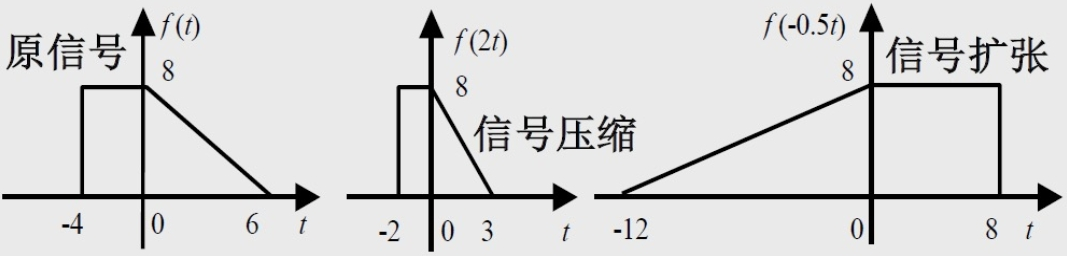
\includegraphics[width=0.5\textwidth]{chap1/img/waveform-scaling.png}
        \caption{信号的压扩运算}
        \label{fig:waveform-scaling}
    \end{figure}
\end{example}

\begin{example}
    已知信号 $f(t)$ 如图 \ref{fig:waveform-exercise-0} 所示,
    请画出 $y(t) = 3f\left(1 - \frac{t}{2}\right) - 1$ 的图形。
    \begin{figure}[H]
        \centering
        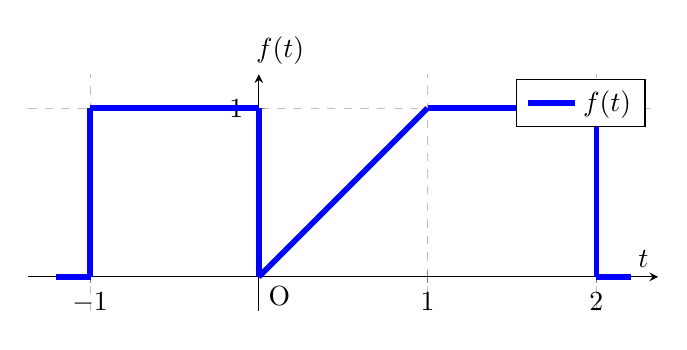
\begin{tikzpicture}
            \begin{axis}[
                axis lines = middle,
                xlabel = {$t$},
                ylabel = {$f(t)$},
                ylabel style={at={(rel axis cs:0.4, 1)}, anchor=south},
                xmin = -1.2, xmax = 2.2,
                ymin = -0.2, ymax = 1.2,
                xtick distance = 1,
                ytick distance = 1,
                grid = major,
                grid style = dashed,
                scale only axis,
                width = 8cm,
                height = 3cm,
                axis equal,
            ]
            \addplot[domain=-1.2:-1, samples=100, smooth, line width=2pt, blue] {0};
            \addplot[smooth, line width=2pt, blue] coordinates {(-1, 0) (-1, 1)};
            \addplot[domain=-1:0, samples=100, smooth, line width=2pt, blue] {1};
            \addplot[smooth, line width=2pt, blue] coordinates {(0, 1) (0, 0)};
            \addplot[domain=0:1, samples=100, smooth, line width=2pt, blue] {x};
            \addplot[domain=1:2, samples=100, smooth, line width=2pt, blue] {1};
            \addplot[smooth, line width=2pt, blue] coordinates {(2, 1) (2, 0)};
            \addplot[domain=2:2.2, samples=100, smooth, line width=2pt, blue] {0};
            \addlegendentry{$f(t)$}
            \node at (axis cs:0,0) [anchor=north west] {O};
            \end{axis}
        \end{tikzpicture}
        \caption{$f(t)$ 的波形描述}
        \label{fig:waveform-exercise-0}
    \end{figure}
\end{example}

\begin{solution}
    首先,对 $f(t)$ 进行时移运算,
    得到 $f\left(1 + t\right)$ 的波形如图 \ref{fig:waveform-exercise-1} 所示。
    \begin{figure}[H]
        \centering
        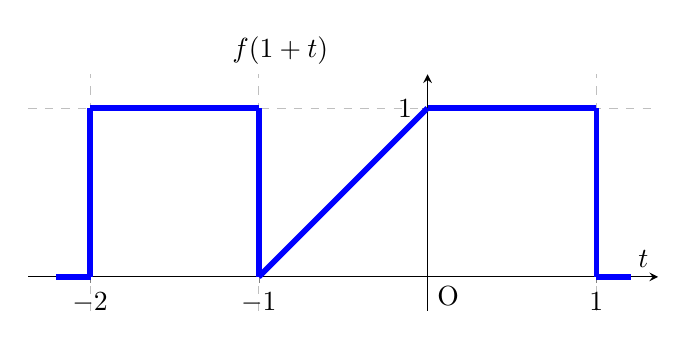
\begin{tikzpicture}
            \begin{axis}[
                axis lines = middle,
                xlabel = {$t$},
                ylabel = {$f(1 + t)$},
                ylabel style={at={(rel axis cs:0.4, 1)}, anchor=south},
                xmin = -2.2, xmax = 1.2,
                ymin = -0.2, ymax = 1.2,
                xtick distance = 1,
                ytick distance = 1,
                grid = major,
                grid style = dashed,
                scale only axis,
                width = 8cm,
                height = 3cm,
                axis equal,
            ]
            \addplot[domain=-2.2:-2, samples=100, smooth, line width=2pt, blue] {0};
            \addplot[smooth, line width=2pt, blue] coordinates {(-2, 0) (-2, 1)};
            \addplot[domain=-2:-1, samples=100, smooth, line width=2pt, blue] {1};
            \addplot[smooth, line width=2pt, blue] coordinates {(-1, 1) (-1, 0)};
            \addplot[domain=-1:0, samples=100, smooth, line width=2pt, blue] {1 + x};
            \addplot[domain=0:1, samples=100, smooth, line width=2pt, blue] {1};
            \addplot[smooth, line width=2pt, blue] coordinates {(1, 1) (1, 0)};
            \addplot[domain=1:1.2, samples=100, smooth, line width=2pt, blue] {0};
            \node at (axis cs:0, 0) [anchor=north west] {O};
            \end{axis}
        \end{tikzpicture}
        \caption{$f(1 - t)$ 的波形描述}
        \label{fig:waveform-exercise-1}
    \end{figure}

    其次,对 $f\left(1 + t\right)$ 进行反褶和压扩运算,
    得到 $f\left(1 - \frac{t}{2}\right)$ 的波形如图 \ref{fig:waveform-exercise-2} 所示。
    \begin{figure}[H]
        \centering
        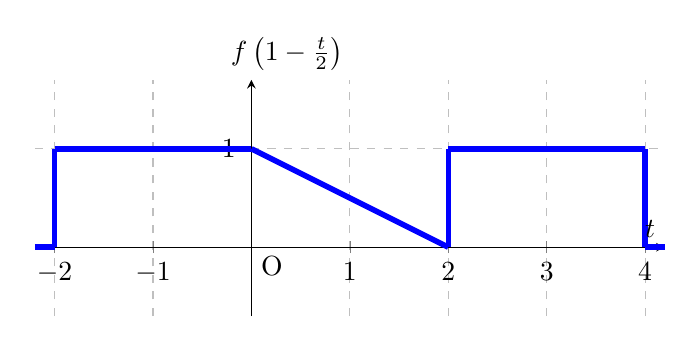
\begin{tikzpicture}
            \begin{axis}[
                axis lines = middle,
                xlabel = {$t$},
                ylabel = {$f\left(1 - \frac{t}{2}\right)$},
                ylabel style={at={(rel axis cs:0.4, 1)}, anchor=south},
                xmin = -2.2, xmax = 4.2,
                ymin = -0.2, ymax = 1.2,
                xtick distance = 1,
                ytick distance = 1,
                grid = major,
                grid style = dashed,
                scale only axis,
                width = 8cm,
                height = 3cm,
                axis equal,
            ]
            \addplot[domain=-2.2:-2, samples=100, smooth, line width=2pt, blue] {0};
            \addplot[smooth, line width=2pt, blue] coordinates {(-2, 0) (-2, 1)};
            \addplot[domain=-2:0, samples=100, smooth, line width=2pt, blue] {1};
            \addplot[domain=0:2, samples=100, smooth, line width=2pt, blue] {1 - 1/2 * x};
            \addplot[smooth, line width=2pt, blue] coordinates {(2, 0) (2, 1)};
            \addplot[domain=2:4, samples=100, smooth, line width=2pt, blue] {1};
            \addplot[smooth, line width=2pt, blue] coordinates {(4, 1) (4, 0)};
            \addplot[domain=4:4.2, samples=100, smooth, line width=2pt, blue] {0};
            \node at (axis cs:0, 0) [anchor=north west] {O};
            \end{axis}
        \end{tikzpicture}
        \caption{$f\left(1 - \frac{t}{2}\right)$ 的波形描述}
        \label{fig:waveform-exercise-2}
    \end{figure}
    
    再次,对 $f\left(1 - \frac{t}{2}\right)$ 进行纵轴方向的缩放和平移,
    得到 $3f\left(1 - \frac{t}{2}\right) - 1$ 的波形如图 \ref{fig:waveform-exercise-3} 所示。
    \begin{figure}[H]
        \centering
        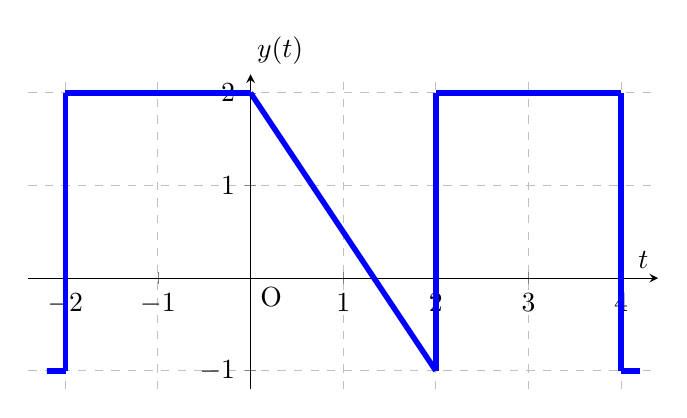
\begin{tikzpicture}
            \begin{axis}[
                axis lines = middle,
                xlabel = {$t$},
                ylabel = {$y(t)$},
                ylabel style={at={(rel axis cs:0.4,1)}, anchor=south},
                xmin = -2.2, xmax = 4.2,
                ymin = -1.2, ymax = 2.2,
                xtick distance = 1,
                ytick distance = 1,
                grid = major,
                grid style = dashed,
                scale only axis,
                width = 8cm,
                height = 4cm,
                axis equal,
            ]
            \addplot[domain=-2.2:-2, samples=100, smooth, line width=2pt, blue] {-1};
            \addplot[smooth, line width=2pt, blue] coordinates {(-2, -1) (-2, 2)};
            \addplot[domain=-2:0, samples=100, smooth, line width=2pt, blue] {2};
            \addplot[domain=0:2, samples=100, smooth, line width=2pt, blue] {2 - 3/2 * x};
            \addplot[smooth, line width=2pt, blue] coordinates {(2, -1) (2, 2)};
            \addplot[domain=2:4, samples=100, smooth, line width=2pt, blue] {2};
            \addplot[smooth, line width=2pt, blue] coordinates {(4, 2) (4, -1)};
            \addplot[domain=4:4.2, samples=100, smooth, line width=2pt, blue] {-1};
            \node at (axis cs:0, 0) [anchor=north west] {O};
            \end{axis}
        \end{tikzpicture}
        \caption{$3f\left(1 - \frac{t}{2}\right)-1$ 的波形描述}
        \label{fig:waveform-exercise-3}
    \end{figure}

\end{solution}

\begin{remark}
    假设有原信号 $y = f(t)$,我们需要画出 $y = Af(\omega t + \varphi) + B$ 的图像时,
    可以按照以下步骤进行:
    \begin{enumerate}
        \item 画出 $y = f(t + \varphi)$ 的图像。
        \item 画出 $y = f(\abs{\omega} t + \varphi)$ 的图像。若 $\omega < 0$ 则再进行反褶(关于 $y$ 轴进行对称)。
        \item 画出 $y = Af(\omega t + \varphi) + B$ 的图像。
    \end{enumerate}
\end{remark}

\begin{note}
    记得标注坐标轴的原点、标注横轴和纵轴的刻度和标识。记得画 $f(t) = 0$ 对应的 $y(t)$ 图像(在上例中,
    对应的是 $(-\infty, -2]$ 和 $[4, +\infty)$ 上的图像 $y = -1$。
\end{note}

\subsubsection{微分与积分运算}

\begin{definition}[信号的能量与功率]
    信号的\bd{能量}和\bd{功率}是描述信号强度的两个重要指标。
    \begin{itemize}
        \item 当信号为连续信号时,信号的\bd{能量}定义为
            \begin{align*}
                E = \int_{-\infty}^{+\infty}\abs{f(t)}^2\D{t},
            \end{align*}
            信号的\bd{功率}定义为
            \begin{align*}
                P = \lim_{T \to +\infty}\frac{1}{2T}\int_{-T}^{T}\abs{f(t)}^2\D{t}.
            \end{align*}
        \item 当信号为离散信号时,信号的\bd{能量}定义为
            \begin{align*}
                E = \sum_{n = -\infty}^{+\infty}\abs{f(n)}^2,
            \end{align*}
            信号的\bd{功率}定义为
            \begin{align*}
                P = \lim_{N \to +\infty}\frac{1}{2N + 1}\sum_{n = -N}^{N}\abs{f(n)}^2.
            \end{align*}
    \end{itemize}
\end{definition}

\begin{definition}[能量信号与功率信号]
    如果信号的能量是有限的,则称为能量有限信号,简称\bd{能量信号}。
    如果信号的功率是有限的,则称为功率有限信号,简称\bd{功率信号}。
\end{definition}

\subsubsection{卷积运算}

\begin{definition}
    设 $f(t), g(t)$ 为两个连续时间信号函数,则它们的\bd{卷积}定义为
    \begin{align*}
        (f * g)(t) = f(t) * g(t) = \int_{-\infty}^{+\infty}f(t - \tau)g(\tau)\D{\tau}.
    \end{align*}

    若 $f(n), g(n)$ 为两个离散时间信号函数,$f, g$ 是 $\set{Z}$ 上的离散序列,
    则它们的\bd{卷积}定义为
    \begin{align*}
        (f * g)(n) = f(n) * g(n) = \sum_{k = -\infty}^{+\infty}f(n - k)g(k).
    \end{align*}
\end{definition}

\begin{remark}
    两个信号的卷积是否存在是有条件的:
    \begin{itemize}
        \item $f, g$ 均为可积函数。
        \item $f, g$ 卷积运算的结果是有界的。
    \end{itemize}
\end{remark}

\begin{note}
    一个信号的反褶信号在 $t$ 轴滑动过程中,
    它与另外一个信号重合部分相乘得到的新信号的面积
    随 $t$ 的变化曲线,就是所求的两个信号的卷积的波形,如图 \ref{fig:convolution-explanation} 所示。
    \begin{figure}[H]
        \centering
        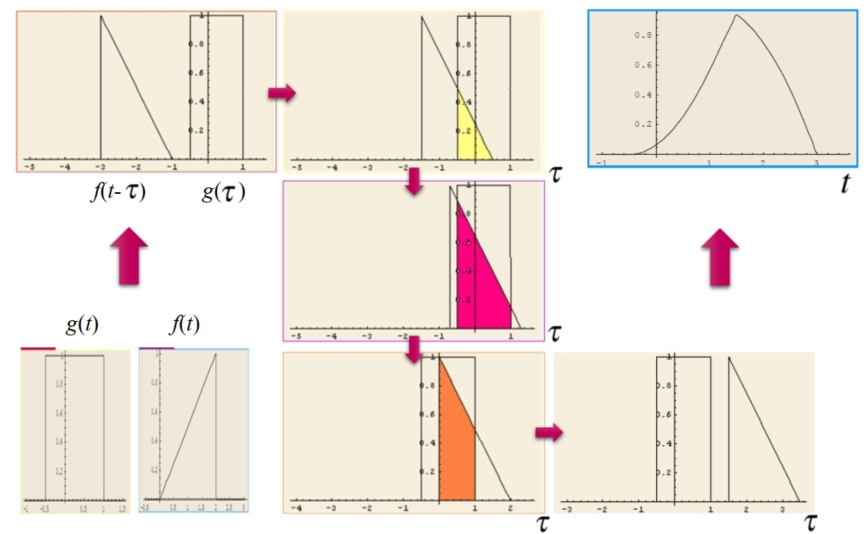
\includegraphics[width=0.5\textwidth]{chap1/img/convolution-explanation.png}
        \caption{卷积运算的解释}
        \label{fig:convolution-explanation}
    \end{figure}
    需要注意的是,卷积不是求图形相交部分的面积,而是求相乘结果的函数的面积。
\end{note}

\begin{property}[卷积运算的交换律]
    卷积运算具有交换律:
    \begin{align*}
        f_1 * f_2 = f_2 * f_1.
    \end{align*}
\end{property}

卷积运算的交换律可以通过变换积分变量的方式来证明。

\begin{proof}
    \begin{align*}
        (f_1 * f_2)(t) & = \int_{-\infty}^{+\infty}f_1(t - a)f_2(a)\D{a} \\
        & = \int_{+\infty}^{-\infty}f_1(b)f_2(t - b)\cdot (-\D{b}) \quad (b = t - a) \\
        & = \int_{-\infty}^{+\infty}f_2(t - b)f_1(b)\D{b} \\
        & = (f_2 * f_1)(t).
    \end{align*}
\end{proof}

\begin{property}[卷积运算的分配律]
    卷积运算具有分配律:
    \begin{align*}
        f_1 * (f_2 + f_3) = f_1 * f_2 + f_1 * f_3.
    \end{align*}
    卷积运算的分配律通常用于并联系统的分析。
\end{property}

卷积运算的分配率可以利用积分运算的线性性来证明。

\begin{proof}
    \begin{align*}
        (f_1 * (f_2 + f_3))(t) & = \int_{-\infty}^{+\infty}f_1(t - a)(f_2(a) + f_3(a))\D{a} \\
        & = \int_{-\infty}^{+\infty}f_1(t - a)f_2(a)\D{a} + \int_{-\infty}^{+\infty}f_1(t - a)f_3(a)\D{a} \\
        & = (f_1 * f_2)(t) + (f_1 * f_3)(t) \\
        & = (f_1 * f_2 + f_1 * f_3)(t).
    \end{align*}
\end{proof}

\begin{property}[卷积运算的结合律]
    卷积运算具有结合律:
    \begin{align*}
        (f_1 * f_2) * f_3 = f_1 * (f_2 * f_3).
    \end{align*}
    卷积运算的结合律通常用于串联系统的分析。
\end{property}

\begin{proof}
    \begin{align*}
        ((f_1 * f_2) * f_3)(t) & = \int_{-\infty}^{+\infty}\left[\int_{-\infty}^{+\infty}f_1(a) f_2(b - a)\D{a}\right]f_3(t - b)\D{b} \\
        & = \int_{-\infty}^{+\infty}f_1(a)\left[\int_{-\infty}^{+\infty}f_2(b - a)f_3(t - b)\D{b}\right]\D{a} \\
        & = \int_{-\infty}^{+\infty}f_1(a)\left[\int_{-\infty}^{+\infty}f_2(c)f_3(t - a - c)\D{c}\right]\D{a}, \quad (c = b - a) \\
        & = \int_{-\infty}^{+\infty}f_1(a)(f_2 * f_3)(t - a)\D{a} \\
        & = (f_1 * (f_2 * f_3))(t).
    \end{align*}
\end{proof}

\begin{property}[卷积的微分性质]
    卷积的微分满足以下性质:两个信号卷积的微分等于其中任一信号的微分与另一信号的卷积,即
    \begin{align*}
        \frac{\D}{\D{t}}\left[f_1(t) * f_2(t)\right]
        = f_1(t) * \frac{\D}{\D{t}}\left[f_2(t)\right]
        = \frac{\D}{\D{t}}\left[f_1(t)\right] * f_2(t),
    \end{align*}
    其中 $f_1, f_2$ 为  $\set{R}$ 上连续可导函数。
\end{property}

\begin{proof}
    \begin{align*}
        \frac{\D}{\D{t}}\left[f_1(t) * f_2(t)\right]
        & = \frac{\D}{\D{t}}\left[\int_{-\infty}^{+\infty}f_1(a) \cdot f_2(t - a)\D{a}\right] \\
        & = \int_{-\infty}^{+\infty}f_1(a) \cdot \frac{\D}{\D{t}}\left[f_2(t - a)\right]\D{a}.
    \end{align*}
    记 $g(t) = \frac{\D}{\D{t}}\left[f_2(t)\right]$,则 $g(t - a) = \frac{\D}{\D{t}}\left[f_2(t - a)\right]$。因此
    \begin{align*}
        \int_{-\infty}^{+\infty}f_1(a) \cdot \frac{\D}{\D{t}}\left[f_2(t - a)\right]\D{a}
        = \int_{-\infty}^{+\infty}f_1(a) \cdot g(t - a)\D{a}
        = f_1(t) * g(t)
        = f_1(t) * \frac{\D}{\D{t}}\left[f_2(t)\right].
    \end{align*}
    同理,由卷积运算的交换律可以证明 $\frac{\D}{\D{t}}\left[f_1(t) * f_2(t)\right] = \frac{\D}{\D{t}}\left[f_1(t)\right] * f_2(t)$。
    因此,命题得证。
\end{proof}

\begin{property}[卷积的积分性质]
    卷积的积分满足以下性质:两个信号卷积的积分等于其中任一信号的积分与另一信号的卷积,即
    \begin{align*}
        \int_{-\infty}^{t}(f_1 * f_2)(\lambda)\D{\lambda}
        = f_1(t) * \left(\int_{-\infty}^{t}f_2(\lambda)\D{\lambda}\right)
        = \left(\int_{-\infty}^{t}f_1(\lambda)\D{\lambda}\right) * f_2(t),
    \end{align*}
    其中 $f_1, f_2$ 为  $\set{R}$ 上连续可导函数。
\end{property}

\begin{proof}
    \begin{align*}
        \int_{-\infty}^{t}(f_1 * f_2)(\lambda)\D{\lambda}
        & = \int_{-\infty}^{t}\left[\int_{-\infty}^{+\infty}f_1(a)f_2(\lambda - a)\D{a}\right]\D{\lambda} \\
        & = \int_{-\infty}^{+\infty}f_1(a)\left[\int_{-\infty}^{t}f_2(\lambda - a)\D{\lambda}\right]\D{a}.
    \end{align*}
    记 $g(t) = \int_{-\infty}^{t}f_2(\lambda)\D{\lambda}$,
    则 $g(t - a) = \int_{-\infty}^{t - a}f_2(\lambda')\D{\lambda'} = \int_{-\infty}^{t}f_2(\lambda - a)\D{\lambda}, \lambda = \lambda' + a$。因此
    \begin{align*}
        \int_{-\infty}^{+\infty}f_1(a)\left[\int_{-\infty}^{t}f_2(\lambda - a)\D{\lambda}\right]\D{a}
        = \int_{-\infty}^{+\infty}f_1(a)g(t - a)\D{a}
        = f_1(t) * g(t)
        = f_1(t) * \left(\int_{-\infty}^{t}f_2(\lambda)\D{\lambda}\right).
    \end{align*}
    同理,由卷积运算的交换律可以证明 $\int_{-\infty}^{t}(f_1 * f_2)(\lambda)\D{\lambda} = \left(\int_{-\infty}^{t}f_1(\lambda)\D{\lambda}\right) * f_2(t)$。
    因此,命题得证。
    
\end{proof}

\begin{corollary}
    设 $f_1, f_2$ 为 $\set{R}$ 上的 $n$ 次可微函数,则
    \begin{align*}
        (f_1 * f_2)^{(n)}(t) = f_1^{(m)}(t) * f_2^{(n - m)}(t), \quad m = 0, 1, \cdots, n.
    \end{align*}
    特别地,当 $n < 0$ 时,记 $f^{(n)}(t)$ 表示对 $f(t)$ 进行 $n$ 次积分运算,则
    \begin{align*}
        (f_1 * f_2)^{(n)}(t) = f_1^{(m)}(t) * f_2^{(n - m)}(t), \quad m = n, n + 1, \cdots, 0.
    \end{align*}
    也就是说,卷积运算的求导次数可以被分配到两个函数上,分别求导后再进行卷积运算;
    积分运算的次数也可以被分配到两个函数上,分别积分后再进行卷积运算。
\end{corollary}

\begin{proof}
    只证明 $n > 0$ 的情况,$n < 0$ 的情况的证明与之类似。使用数学归纳法证明。
    
    当 $n = 1$ 时,由卷积的微分性质即可得证。假设 $n = k$ 时结论成立,即
    \begin{align*}
        (f_1 * f_2)^{(k)}(t) = f_1^{(m)}(t) * f_2^{(k - m)}(t), \quad m = 0, 1, \cdots, k.
    \end{align*}
    当 $n = k + 1$ 时,有
    \begin{align*}
        (f_1 * f_2)^{(k + 1)}(t) & = \frac{\D}{\D{t}}\left[(f_1 * f_2)^{(k)}(t)\right] \\
        & = \frac{\D}{\D{t}}\left[f_1^{(m)}(t) * f_2^{(k - m)}(t)\right] \\
        & = f_1^{(m + 1)}(t) * f_2^{(k - m)}(t) \\
        & = f_1^{(m)}(t) * f_2^{(k - m + 1)}(t).
    \end{align*}
    因此,由数学归纳法可知,对于任意的 $n \ge 0$,结论均成立。
\end{proof}

\subsubsection{相关运算}

\begin{definition}
    两个信号的\bd{相关运算}定义为
    \begin{align*}
        R_{f_1, f_2}(t)
        = R(f_1(t), f_2(t))
        = \int_{-\infty}^{+\infty}f_1(\tau)f_2^*(\tau - t)\D{\tau}
        = \int_{-\infty}^{+\infty}f_1(\tau + t)f_2^*(\tau)\D{\tau}.
    \end{align*}
    可以看出,$f_1$ 和 $f_2^*$ 在乘法运算时有一个相对平移量 $t$。
\end{definition}

\begin{remark}
    相关运算和卷积运算有一定的联系:$R_{f_1, f_2}(t) = f_1(t) * f_2^*(-t)$,
    但也有一定的区别:相关运算中的第二个信号\bd{不需要反褶},但\bd{需要取共轭}。
\end{remark}

\begin{property}
    信号的相关运算与顺序有关。考虑 $R_{f_2, f_2}(t)$:
    \begin{align*}
        R_{f_2, f_1}(t) = R(f_2(t), f_1(t)) = \int_{-\infty}^{+\infty}f_2(\tau)f_1^*(\tau - t)\D{\tau}.
    \end{align*}
    对比 $R_{f_1, f_2}(t)$,可以发现
    \begin{align*}
        R_{f_2, f_1}(t) & = \int_{-\infty}^{+\infty}f_1(a)f_2^*(a - t)\D{a} \\
        & = \left[\int_{-\infty}^{+\infty}f_1^*(a)f_2(a - t)\D{a}\right]^* \\
        & = R_{f_1, f_2}^*(-t).
    \end{align*}
\end{property}

\begin{note}
    \begin{align*}
        f_1(t) * f_2(t) & = \int_{-\infty}^{+\infty}f_1(t - a)f_2(a)\D{a}, \\
        f_1(-t) * f_2(t) & = \int_{-\infty}^{+\infty}f_1(a - t)f_2(a)\D{a} \\
        & \neq \int_{-\infty}^{+\infty}f_1(-t - a)f_2(a)\D{a}.
    \end{align*}
    一个比较容易的方法,是记 $g(t) = f_1(-t)$,
    这样 $g(t) * f_2(t) = \int_{-\infty}^{+\infty}g(t - a)f_2(a)\D{a} = \int_{-\infty}^{+\infty}f_1(a - t)f_2(a)\D{a}$,
    就不会记错了。
\end{note}

\begin{example}[自相关运算]
    自相关运算是指函数自己与自己求相关。用自相关函数可以检测准周期信号的准周期,
    如图 \ref{fig:self-relation} 所示。
    \begin{figure}[H]
        \centering
        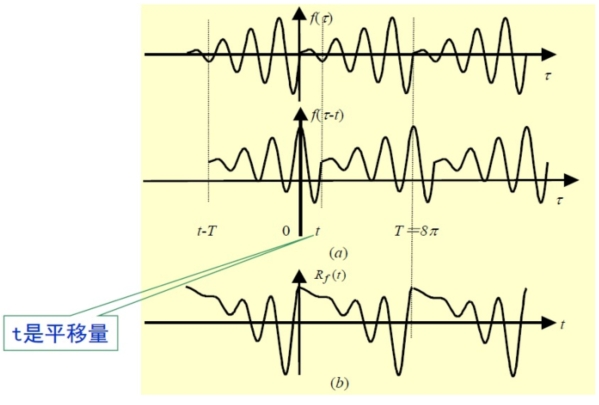
\includegraphics[width=0.5\textwidth]{chap1/img/self-relation.png}
        \caption{函数的自相关运算}
        \label{fig:self-relation}
    \end{figure}
\end{example}

\begin{example}[卷积的物理意义]
    设 $g(x, y)$ 表示图像,$f(x, y)$ 表示卷积核。则如图 \ref{fig:graph-convolution-example-1} 和
    图 \ref{fig:graph-convolution-example-2} 所示,
    \begin{figure}[H]
        \centering
        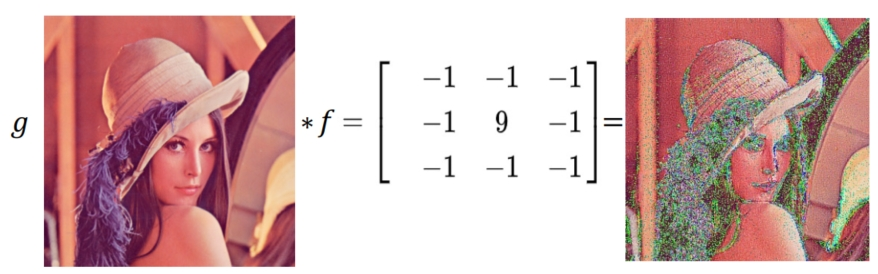
\includegraphics[width=0.5\textwidth]{chap1/img/graph-convolution-example-1.png}
        \caption{卷积的物理意义(1)}
        \label{fig:graph-convolution-example-1}
    \end{figure}
    为何``积''?``积''的过程中,我们得到了一个叠加值,我们通过定义 $f$,使得叠加值包含图像的特定信息,例如边缘信息,平滑处理。
    \begin{figure}[H]
        \centering
        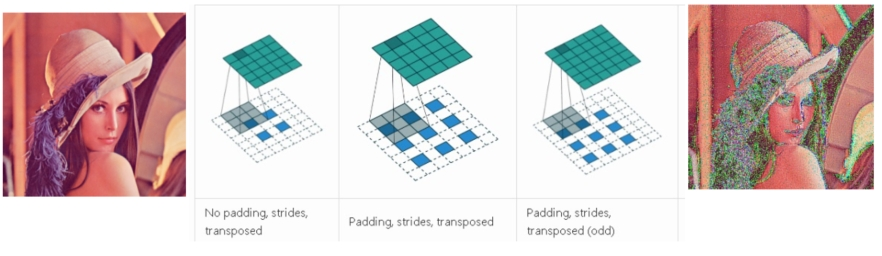
\includegraphics[width=0.5\textwidth]{chap1/img/graph-convolution-example-2.png}
        \caption{卷积的物理意义(2)}
        \label{fig:graph-convolution-example-2}
    \end{figure}
\end{example}

\begin{note}
    卷积的定义中,为何要对 $f$ 做反褶?为了数学上的便利性,反褶后卷积可以满足交换律;
    另一方面,在后续的学习中,我们会发现时域的卷积在频域上有很简洁的形式。
\end{note}
